\section{Using functions with different numbers of parameters (5 pages)}
\label{sec:correction}

\subsection{Corrections to 2NLL}
\label{sec:correction:corrections}

The 2NLL calculated from the fit of a function to a dataset is purely a measure
of the agreement of the function and the data; the number of parameters
used in the function has no impact. Hence, at least for nested families of
functions (such as polynomials of varying order), then the lowest 2NLL will
always be given by the highest order considered.
Because this function also has the
largest number of parameters, it will generally have the largest statistical
error and hence widest 2NLL profile curve.
Hence, simply using the 2NLL values
without any ``penalty'' for the number of parameters would effectively
always result in the minimum envelope being mainly defined by the highest
order function. It would also mean there is no ``natural'' way to know when
to no longer consider yet more higher order functions. However, tests such as
the F-test are standardly used to determine when higher order functions in
a family can be ignored. Hence, when using functions with different
numbers of parameters, it seems necessary to have some correction to the 2NLL
value to account for this difference in number.

The idea is therefore to compare 2NLL values,
correcting for the differing number of parameters 
(or equivalently differing number of degrees of freedom) in
the fit functions. Specifically here, where applied, the correction is
done so as to get a value equivalent to a function with no parameters, so
the number of degrees of freedom is the number of bins used.
Two obvious methods were considered, based on the 
$\chi^2$ p-value and the Akaike information 
criterion~\cite{ref:correction:akaike}.
\begin{enumerate}
\item[p-value]
For a binned fit using the expression for the 2NLL ratio
for each bin specified in equation~\ref{eqn:introduction:def2NLL}, then for
the large statistics case, the 2NLL becomes equivalent to a $\chi^2$ for the
fit. In this case, it is meaningful to find the p-value of the $\chi^2$ value.
A new $\chi^{\prime 2}$
value can now be obtained, namely that which would give the same p-value but
with a different number of degrees of freedom, equal to the number of bins.
The corrected 2NLL is then given by
\begin{displaymath}
C = \chi^{\prime 2} = - 2\ln(L) + (\chi^{\prime 2} - \chi^2)
\end{displaymath}
Besides being a function of the number of bins and parameters,
the size of the correction $\chi^{\prime 2} - \chi^2$
depends on the original fit quality
(or equivalently p-value). Figure~\ref{fig:correction:DeltaChiSq}
shows examples of the size of the correction as a function of the
fit p-value, when correcting for various numbers of parameters.
The correction is monotonically increasing as the p-value gets smaller.
Hence, when correcting the 2NLL profile curve, the fits further away from
the best fit minimum will get a larger correction. Hence, the profile curve
becomes steeper, which could in principle affect the coverage.
%Figure~\ref{fig:parameters:pvalue} shows the effect of the correction
%for the power-law fit on the profile
%(shown uncorrected in figure~\ref{fig:nuisance:powfit})
%and on the Neymann fraction
%(shown uncorrected in figure~\ref{fig:nuisance:powfraction}).
%In both cases, the effect of the correction is almost negligible
%in practice.
However, it can be seen that the correction is approximately given by
\begin{displaymath}
\chi^{\prime 2} - \chi^2 \approx N_{\rm par}
\end{displaymath}
for the central range of p-values. This approximation means the 
2NLL shape, and hence coverage, is unchanged and this is used in the rest
of this paper.
%
\begin{figure}[tbp]
\centering
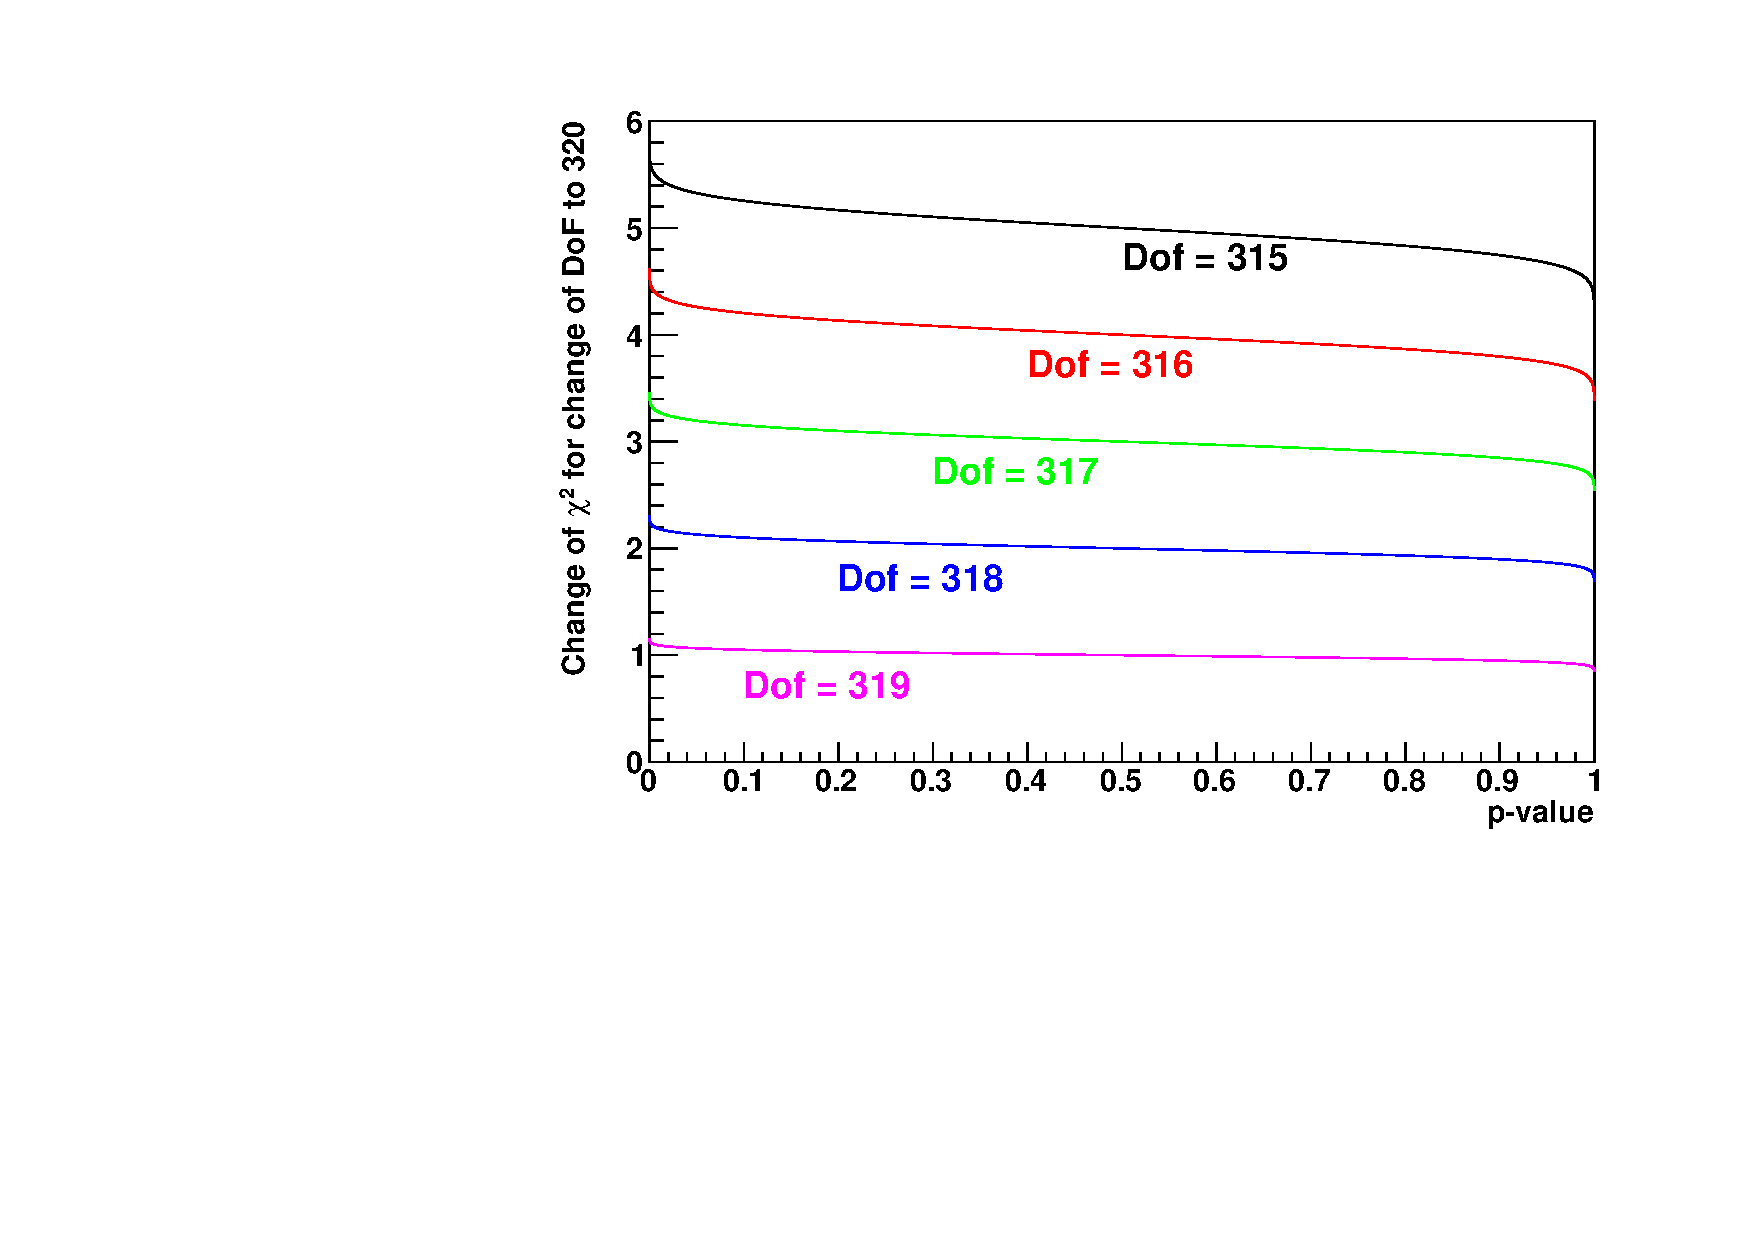
\includegraphics[width=0.45\textwidth]{correction/DeltaChiSq1.pdf}
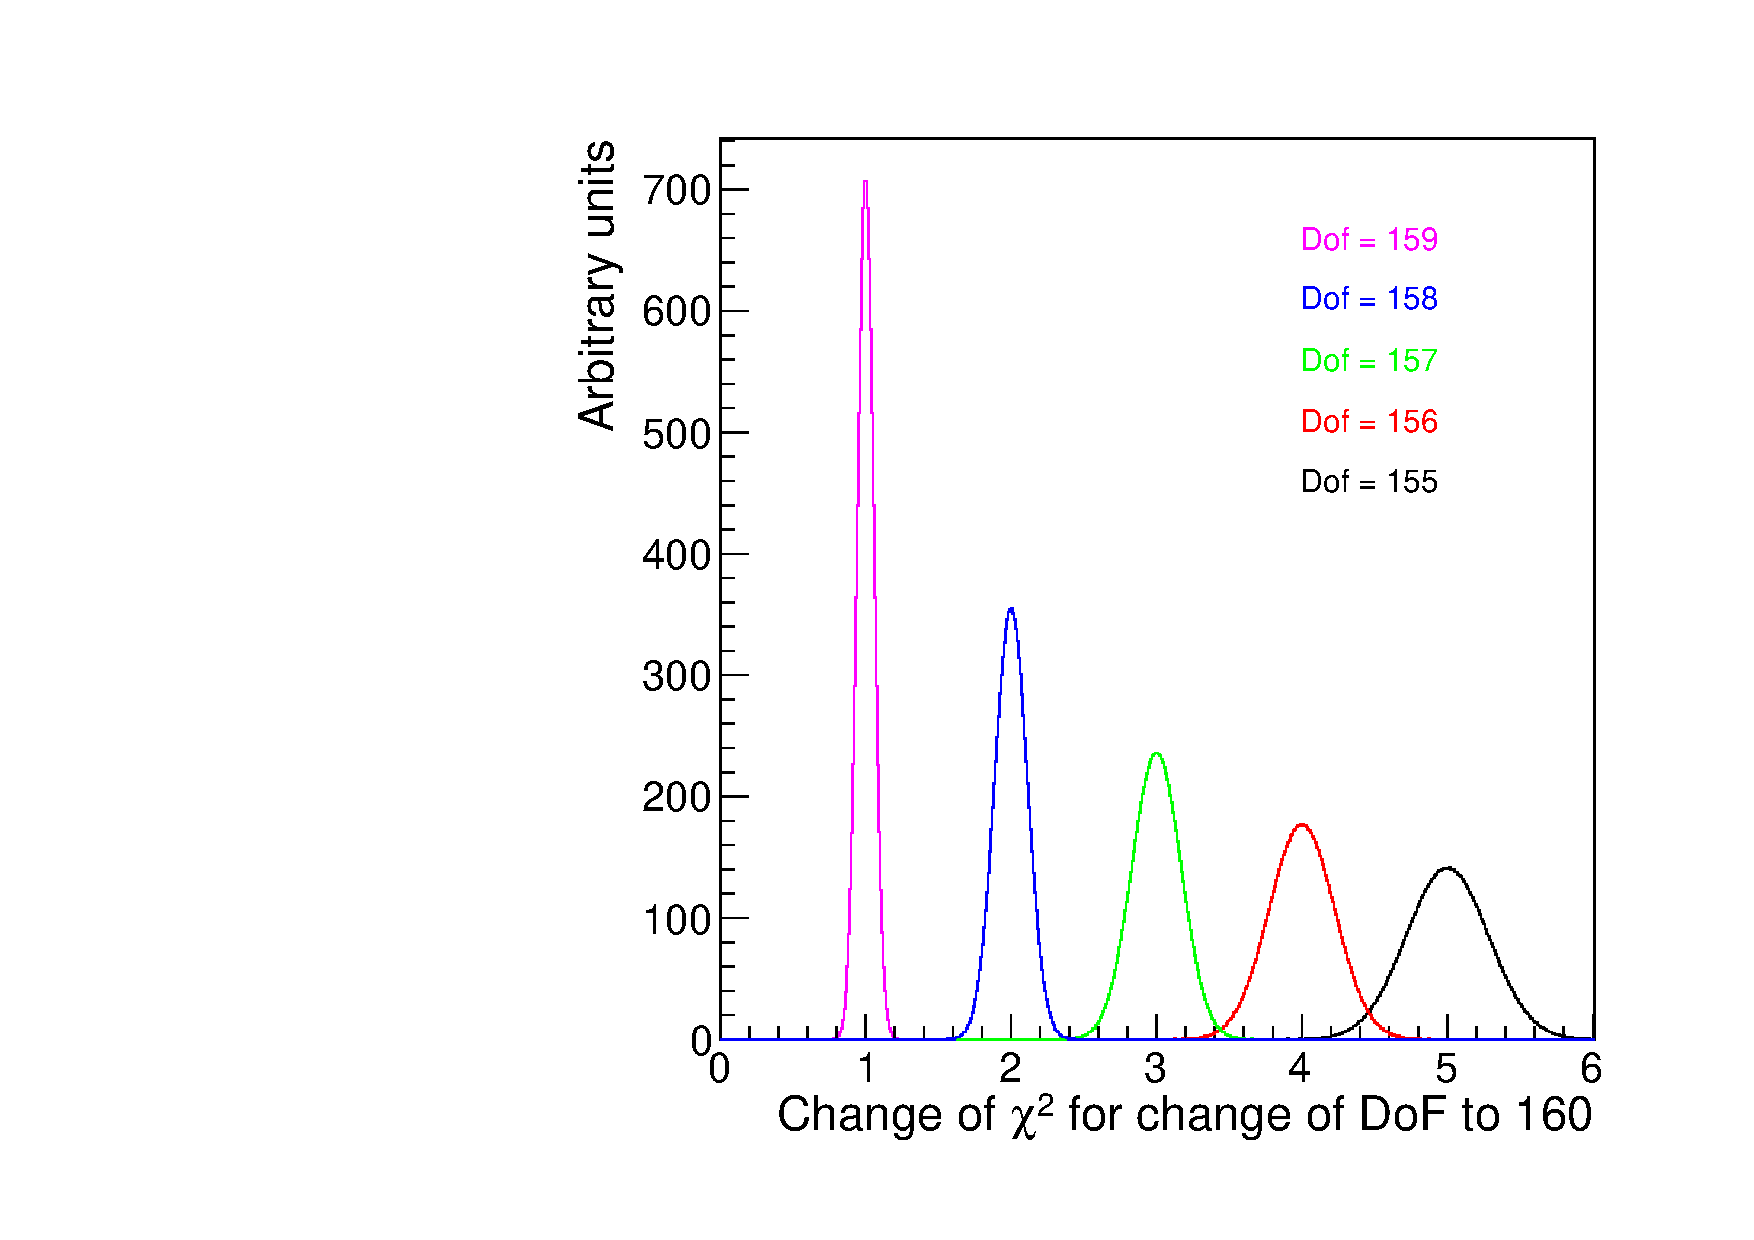
\includegraphics[width=0.45\textwidth]{correction/DeltaChiSq2.pdf}
\caption{Change of $\chi^2$ when correcting for between one and five parameters
in a fit with 320 bins. The change to the $\chi^2$ as a function of the
original p-value is shown on the left. The distribution of the change of
the $\chi^2$ assuming a flat p-value distribution is shown on the right.}
\label{fig:correction:DeltaChiSq}
\end{figure}


\item[Akaike]
The Akaike basic formula for very large sample sizes is
\begin{displaymath}
A = - 2\ln(L) + 2N_{\rm par}
\end{displaymath}
The resulting value of $A$ is considered here as the corrected 2NLL,
so the correction is simply $ 2N_{\rm par}$ and
hence is twice as big as the p-value correction.
For finite samples, then it is modified to
\begin{displaymath}
A 
= - 2\ln(L) + 2N_{\rm par}  + \frac{2N_{\rm par}(N_{\rm par}+1)}{n-(N_{\rm par}+1)}
= - 2\ln(L) + \frac{2N_{\rm par}}{1-(N_{\rm par}+1)/n}
\end{displaymath}
where $n$ is the sample size, i.e. the number of bins (for a binned likelihood
fit) or events (for an unbinned likelihood fit). For large $n$, the original
formula is clearly regained. This can be used for binned or unbinned fits.
Also the correction does not depend on the 2NLL value and
so is a simple shift of
the whole profile curve, without changing its shape.
Hence, it also has no effect on coverage.
\end{enumerate}

\subsection{Function definitions}
\label{sec:correction:functions}
DESCRIBE THE RECURSIVE FRACTION DEFINITIONS USED HERE AND WHICH ONES WE USE
\subsection{Example case}
\label{sec:correction:example}

SHOWING RESULTS USING CORRECTION 1 PER DOF. SHOULD WE COMPARE TO AKAIKE AND PVALUE BASED CORRECTION?

When including higher order functions, the 95.4\% confidence interval on $\mu$ is extended 
due to the influence of the higher order polynomial functions providing a reasonable 
description of the data. The central value is unchanged since the lowest order power law 
best desribes the data when including a penalty for using additional parameters in the fit.

\begin{figure}[tbp]
\centering
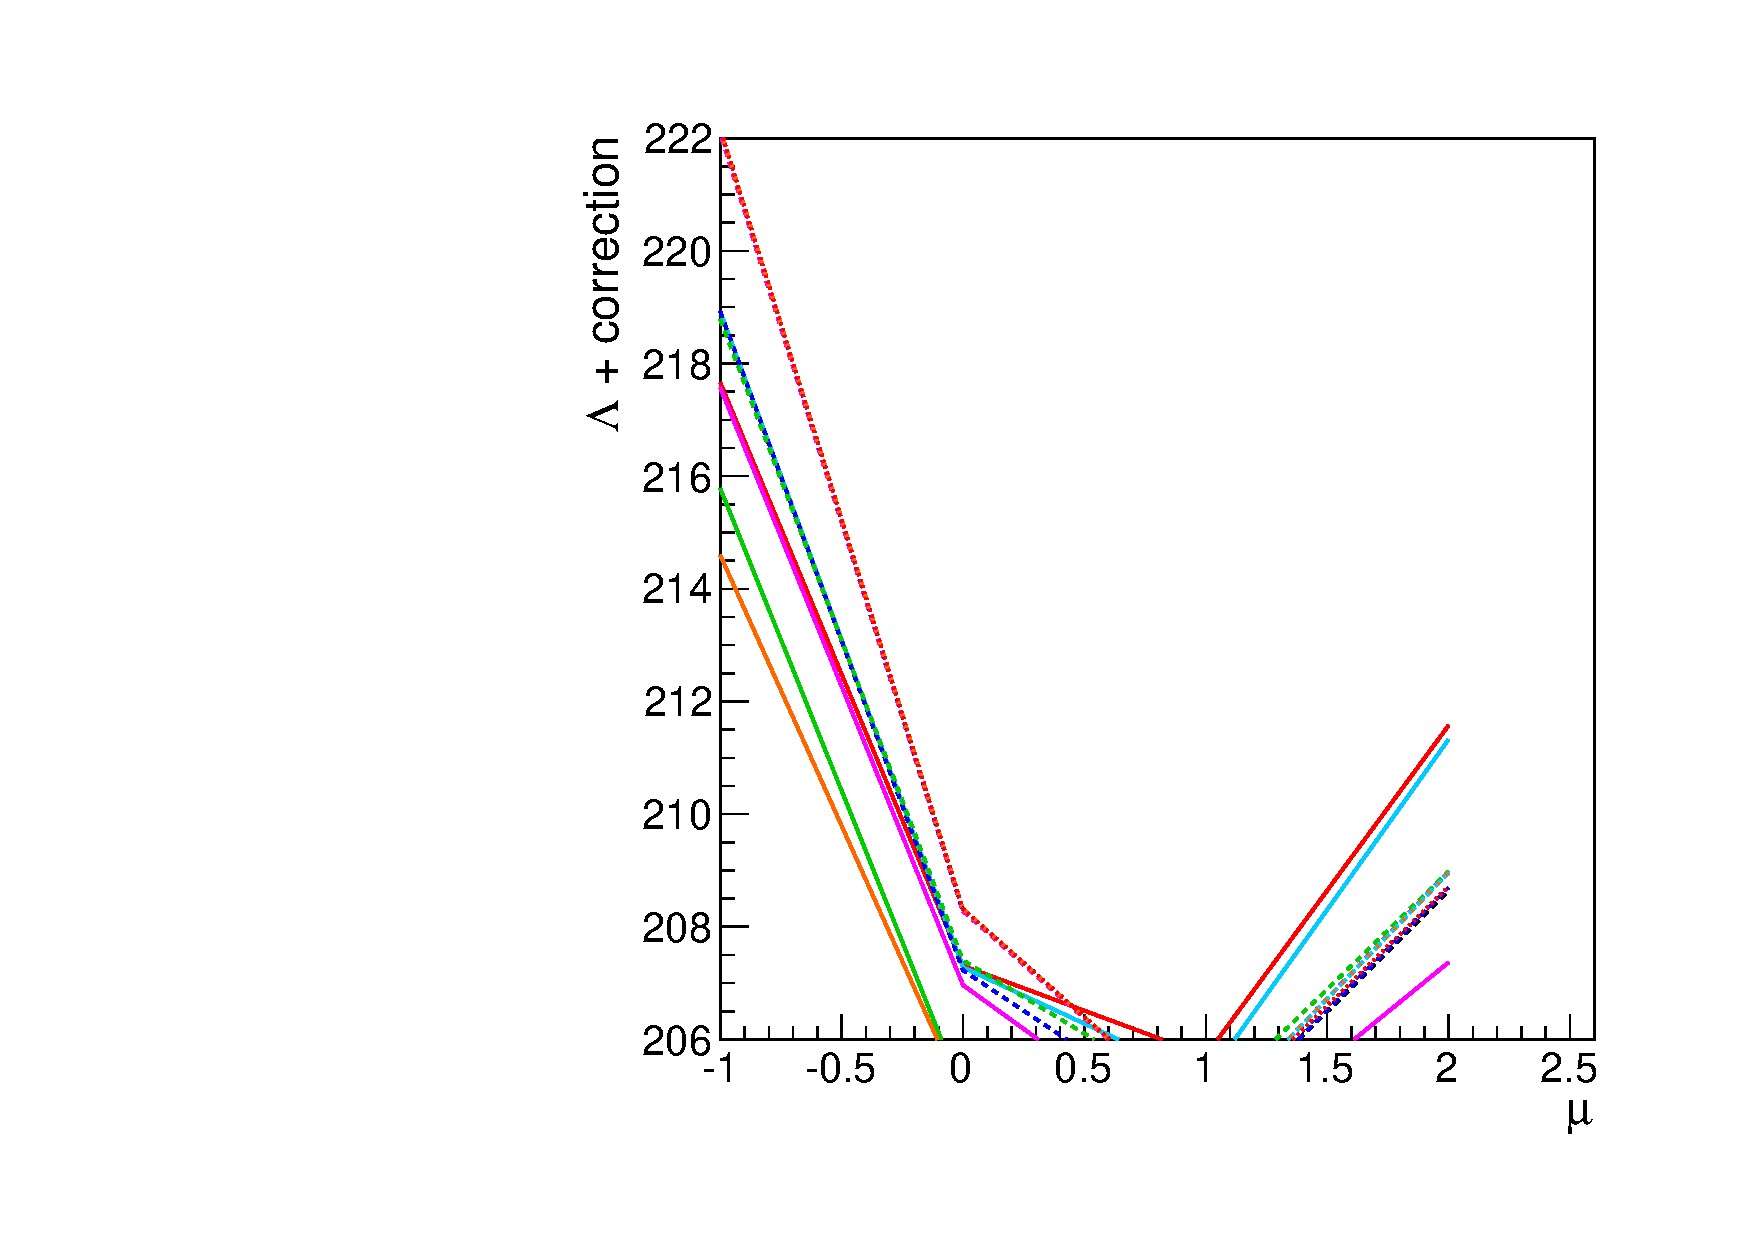
\includegraphics[width=0.45\textwidth]{correction/ProfilesAllOrders.pdf}
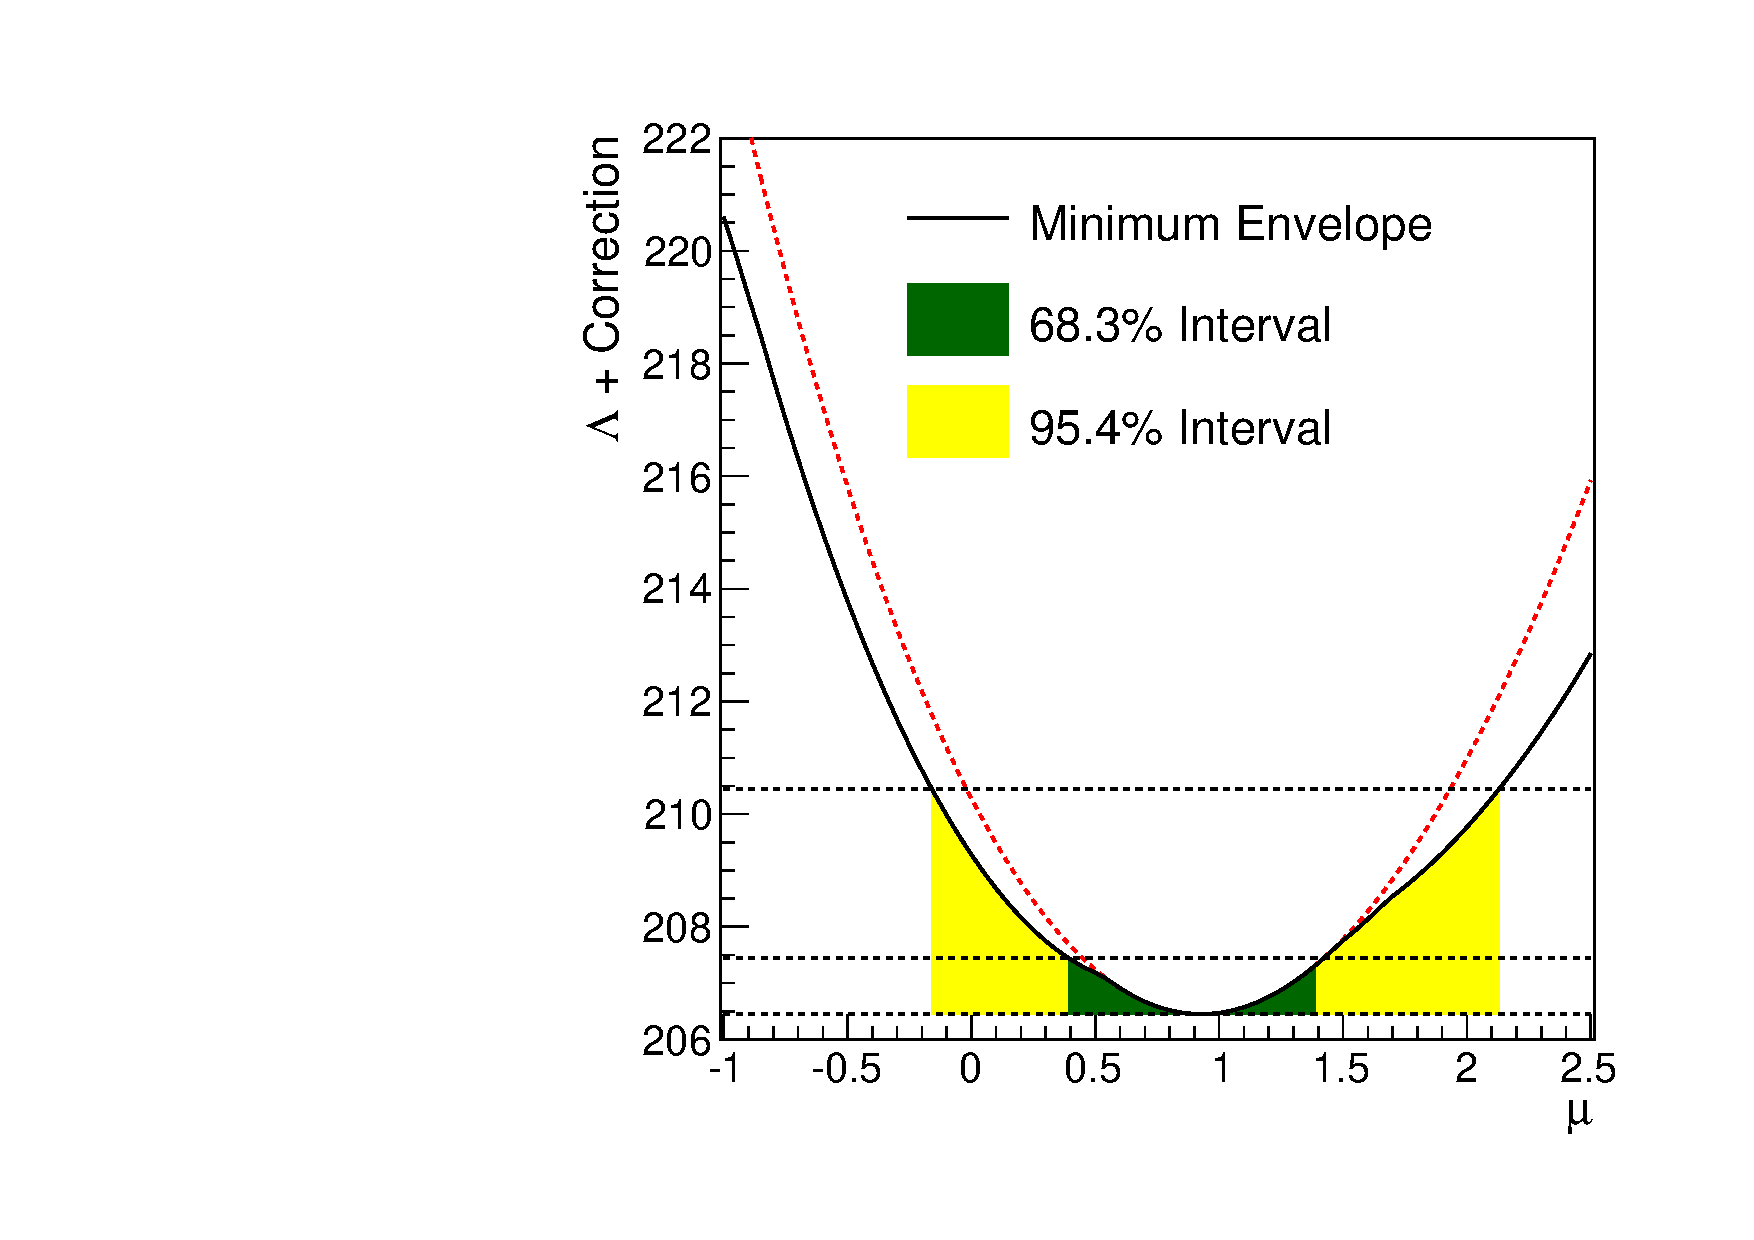
\includegraphics[width=0.45\textwidth]{correction/EnvelopeAllOrders.pdf}
\caption{Left: Profile 2NLL scans for all of the functions considered. The 2NLL values for
each profile has been corrected by 1 unit per background function parameter. 
Right: Minimum envelope of the functions onsidered accounting for the correction of 1 per 
background parameter. The 2NLL scan when only considering the lowest order power law function 
is shown in red.}
\label{fig:correction:profiles}
\end{figure}


%RELATION TO BIAS WHEN USING FUNCTION A TO FIT FUNCTION B? ASIMOV?

%\subsection{Toy generation}
%\label{sec:correction:toys}

%EXTRA COMPLICATION WITH BAYESIAN AND FREQUENTIST MIXTURES OF NORMALISATION

\subsection{Bias and coverage depoendence on correction}
\label{sec:correction:bias}

\begin{figure}[tbp]
\centering
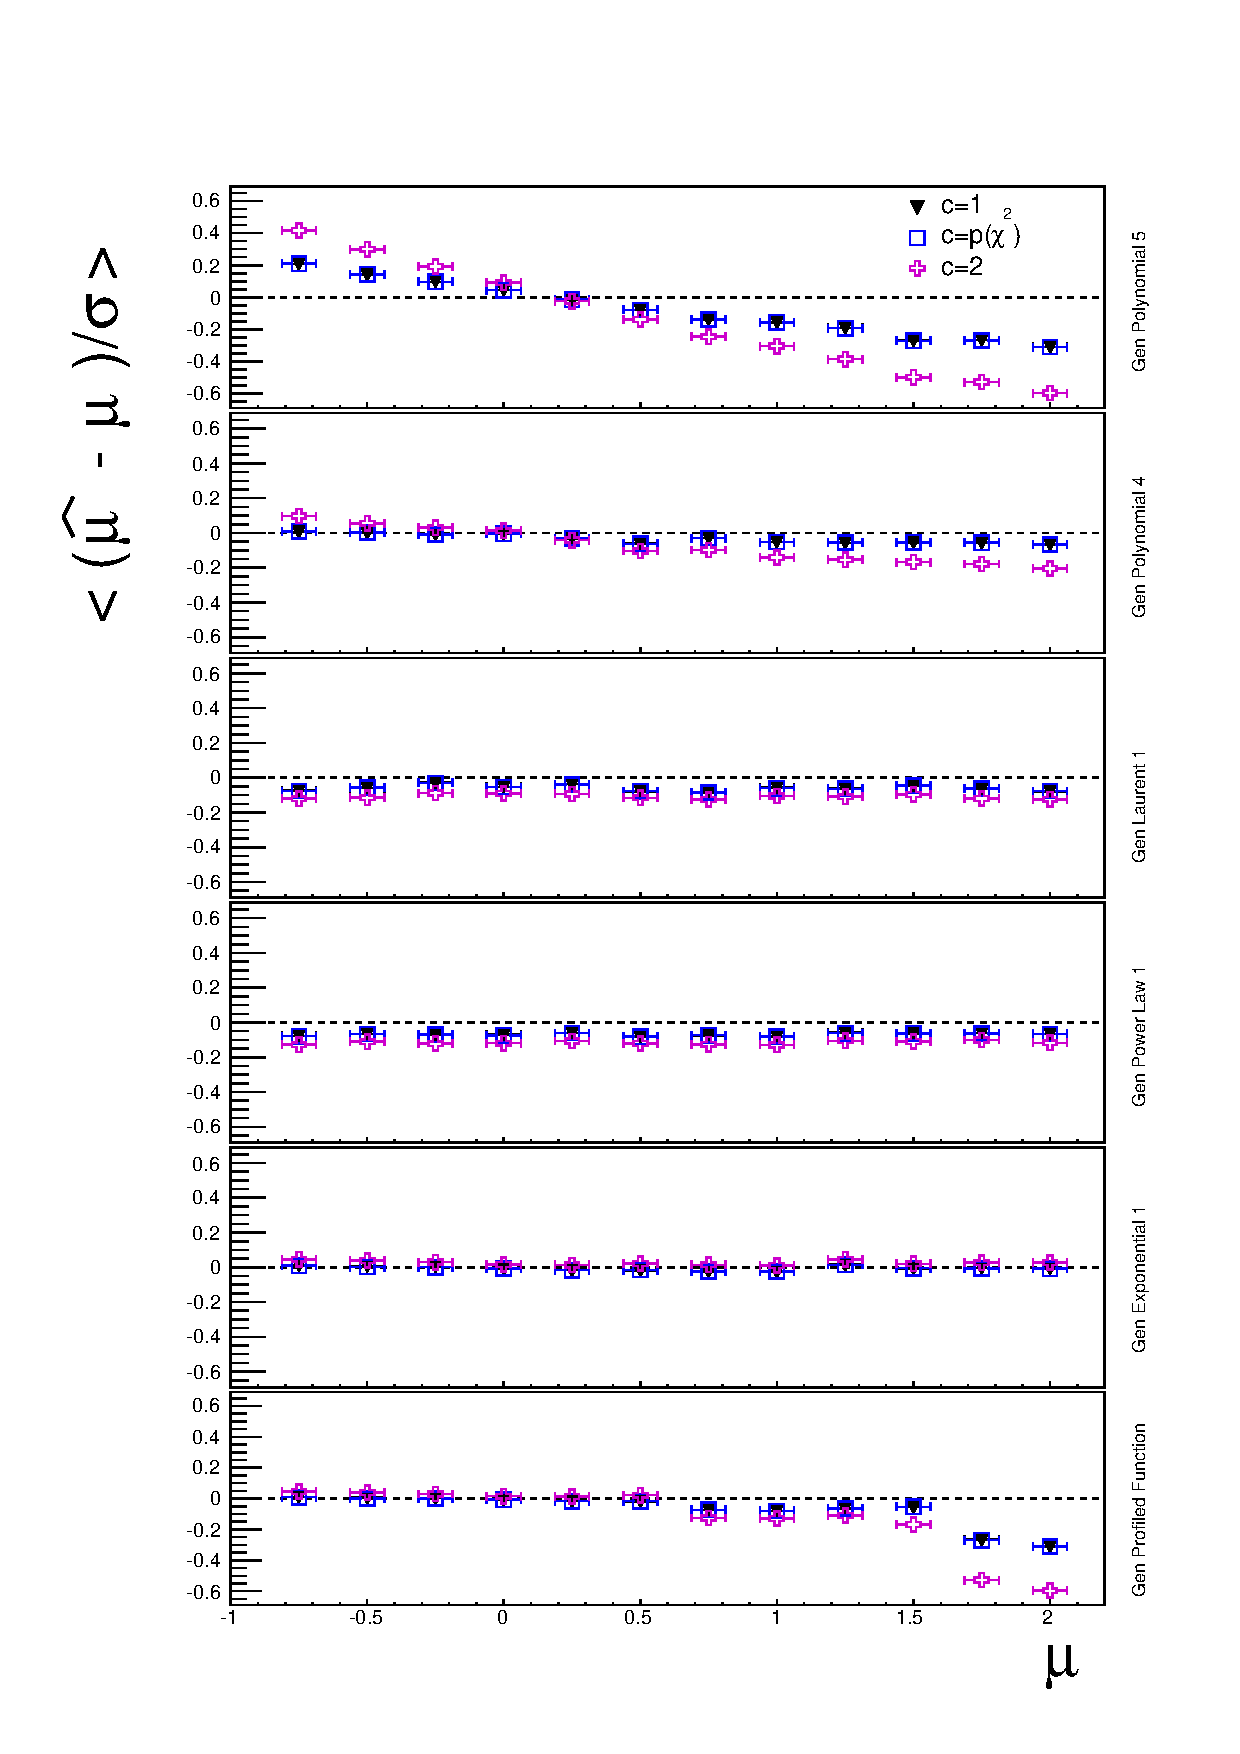
\includegraphics[width=0.45\textwidth]{correction/AllOrderFunctions_call.pdf}
\caption{Average pull when fitting using the envelope as a function of $\mu$ 
used to generate the signal. Each panel shows the average bias when using 
a different background function for toy generation.
The top plot show the result when the best-fit function at each
value of $\mu$ is used to generate toys.}
\label{fig:correction:allorderbias}
\end{figure}


\begin{figure}[tbp]
\centering
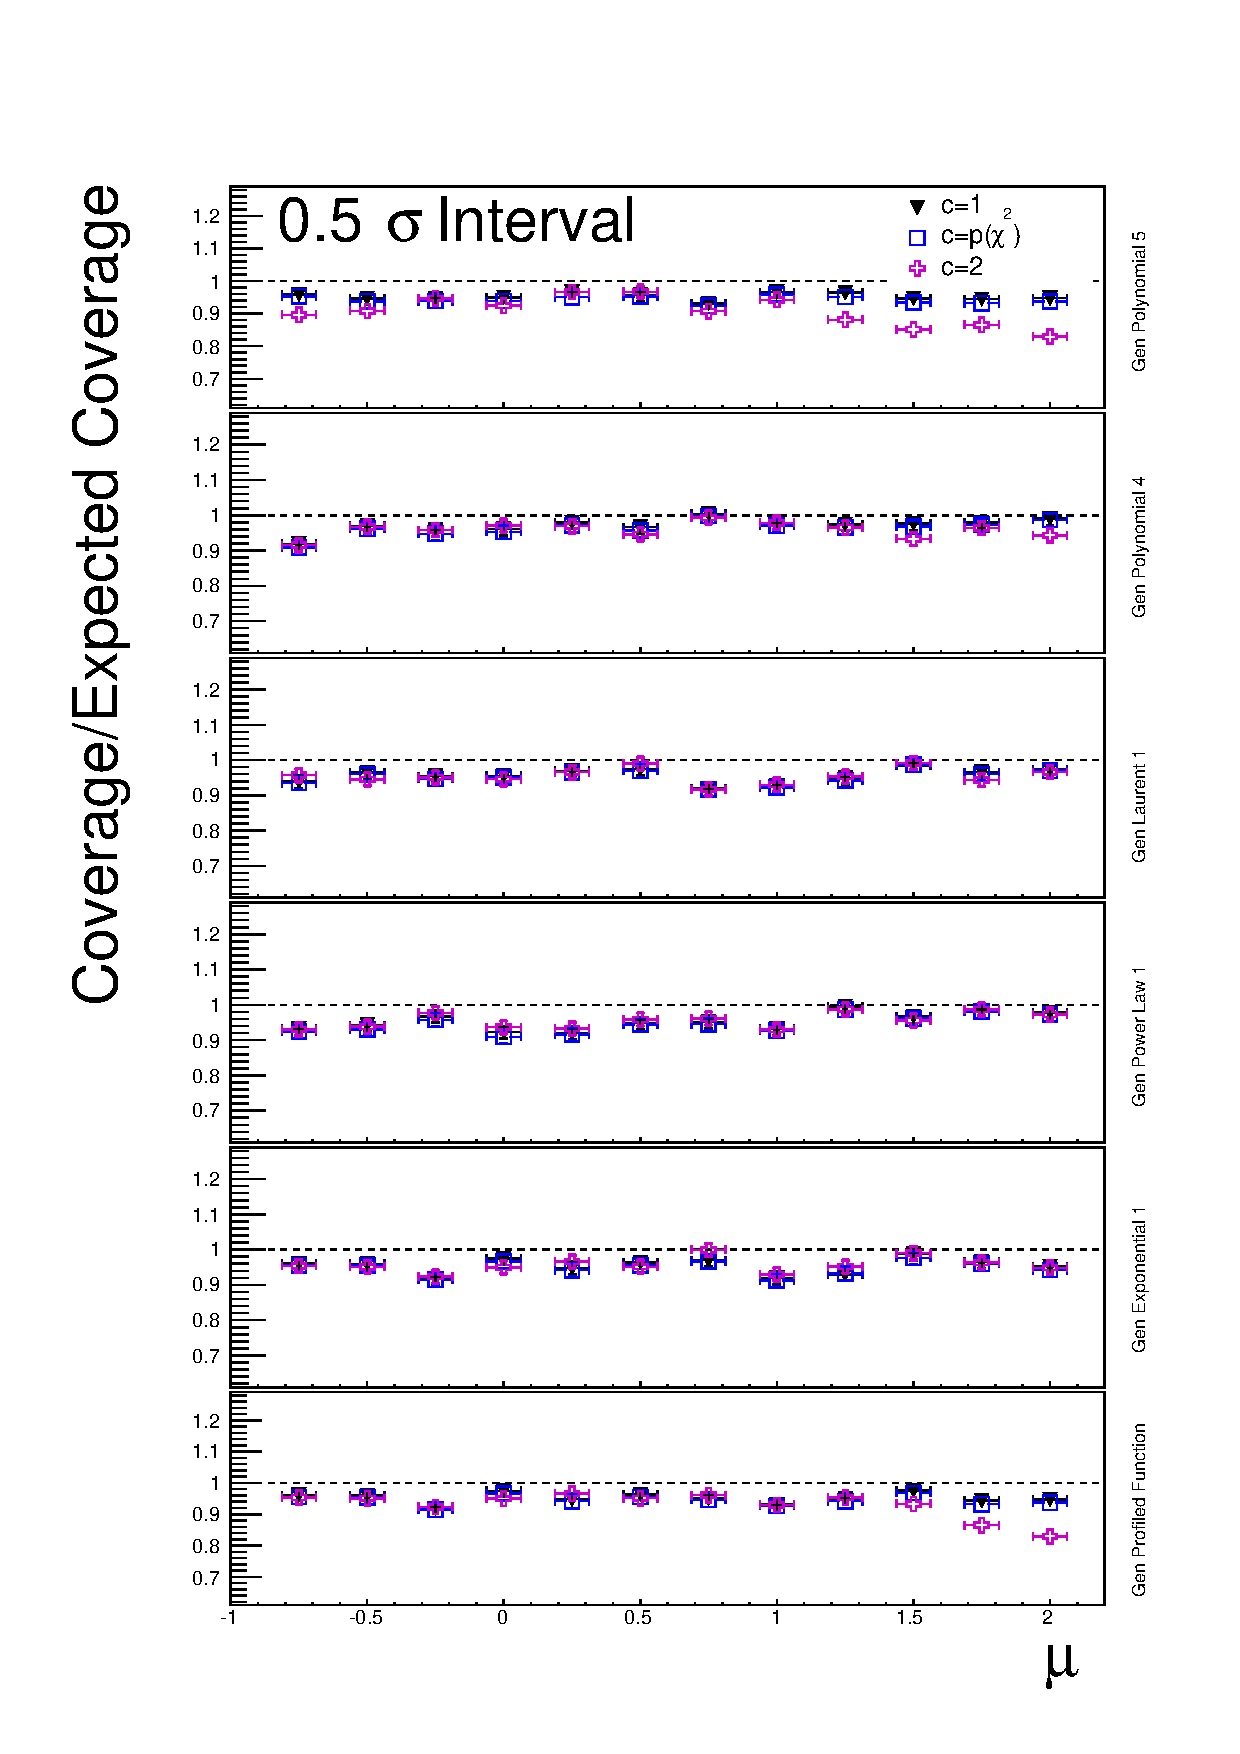
\includegraphics[width=0.45\textwidth]{{correction/AllOrderFunctions_Coverage_0.5_call}.pdf}
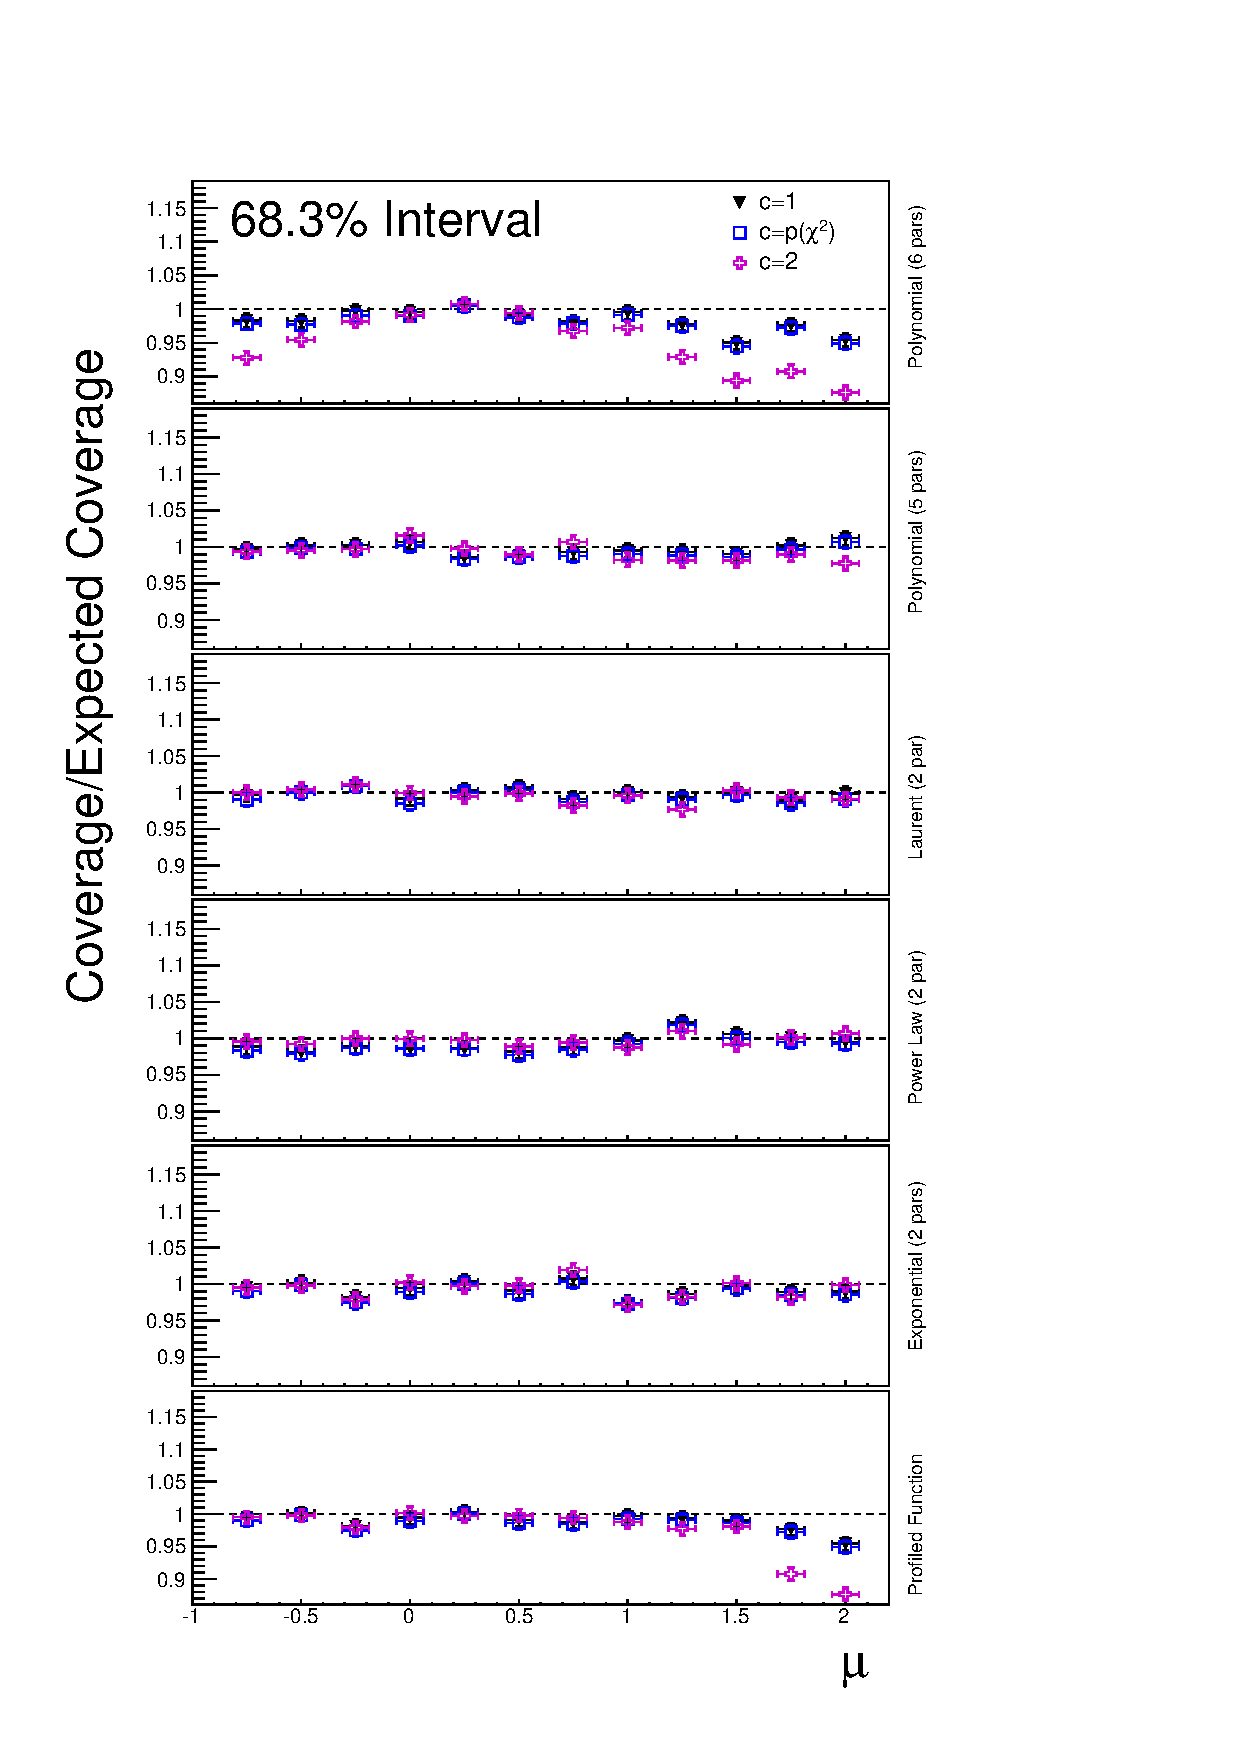
\includegraphics[width=0.45\textwidth]{{correction/AllOrderFunctions_Coverage_1._call}.pdf}\\
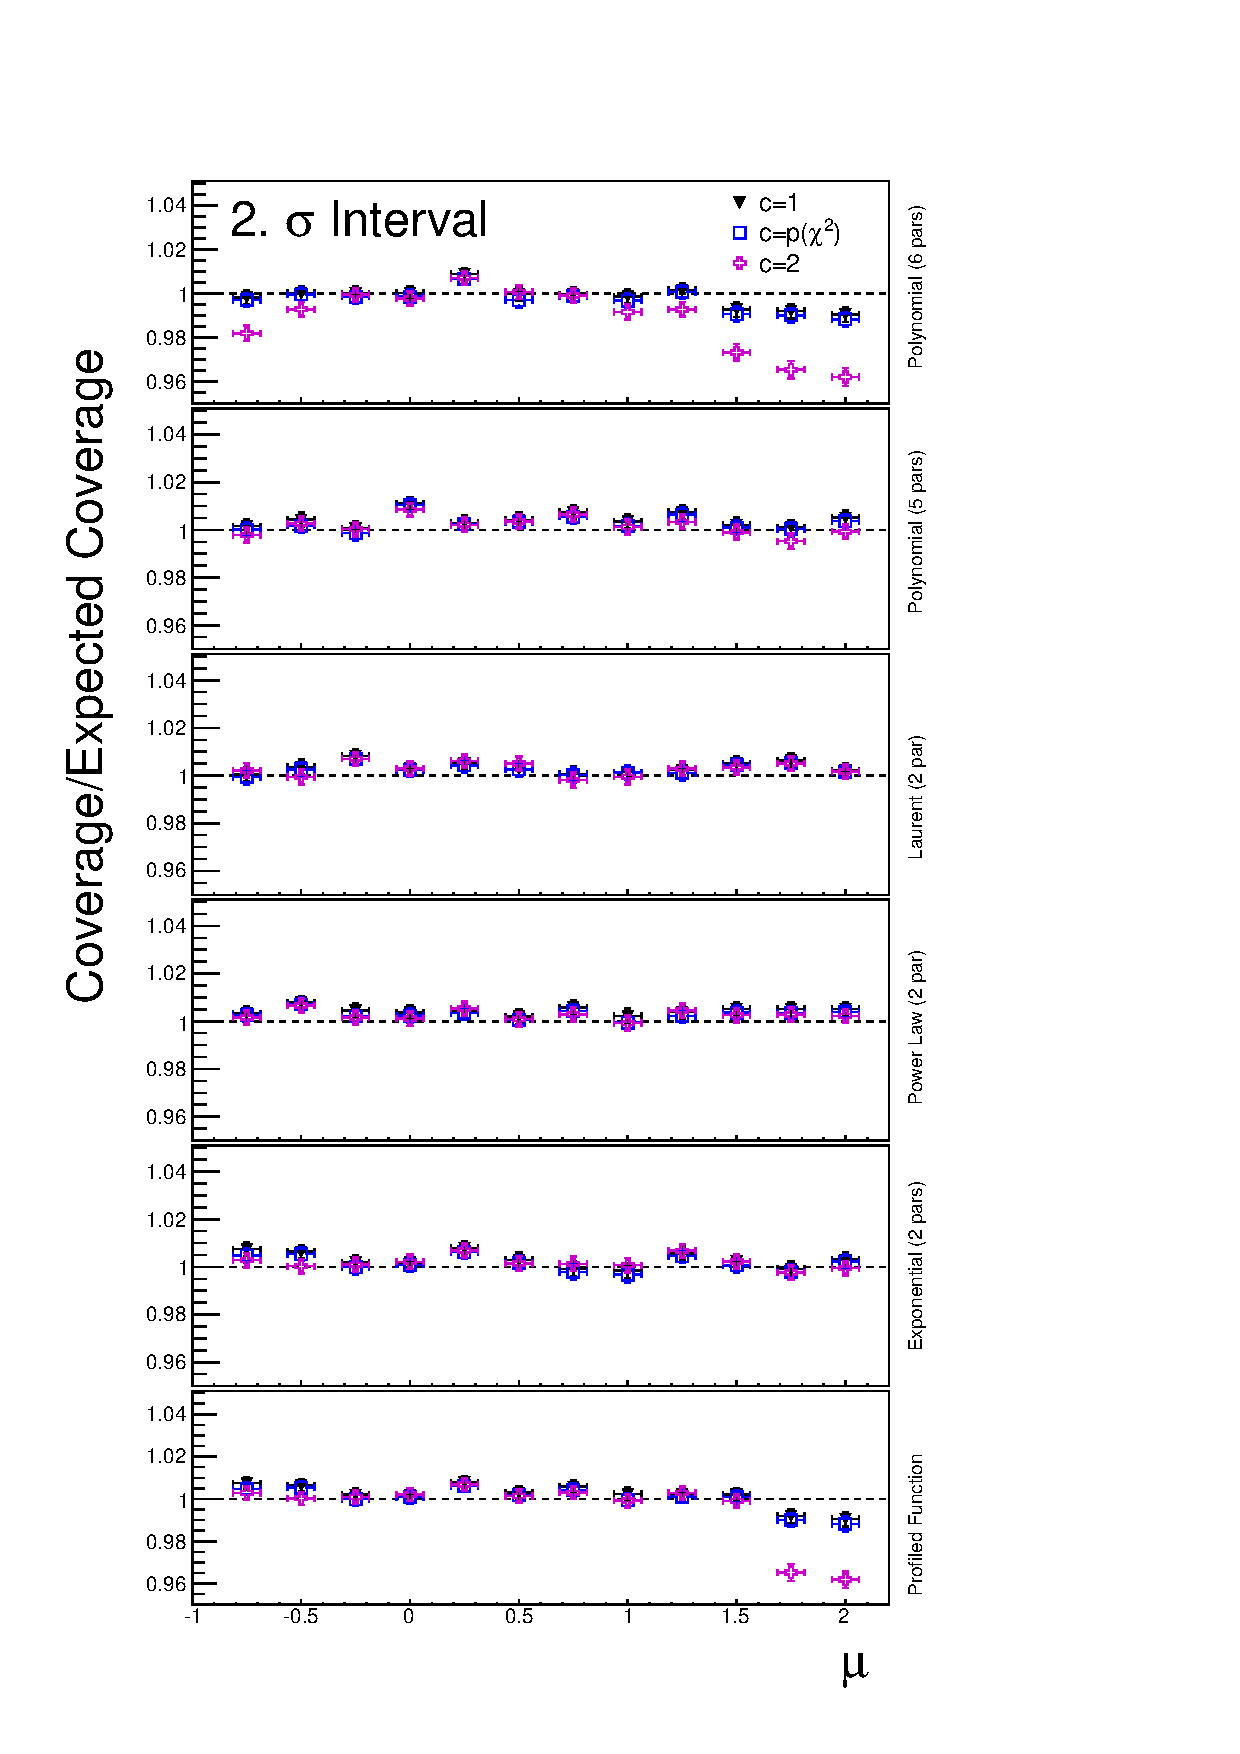
\includegraphics[width=0.45\textwidth]{{correction/AllOrderFunctions_Coverage_2._call}.pdf}
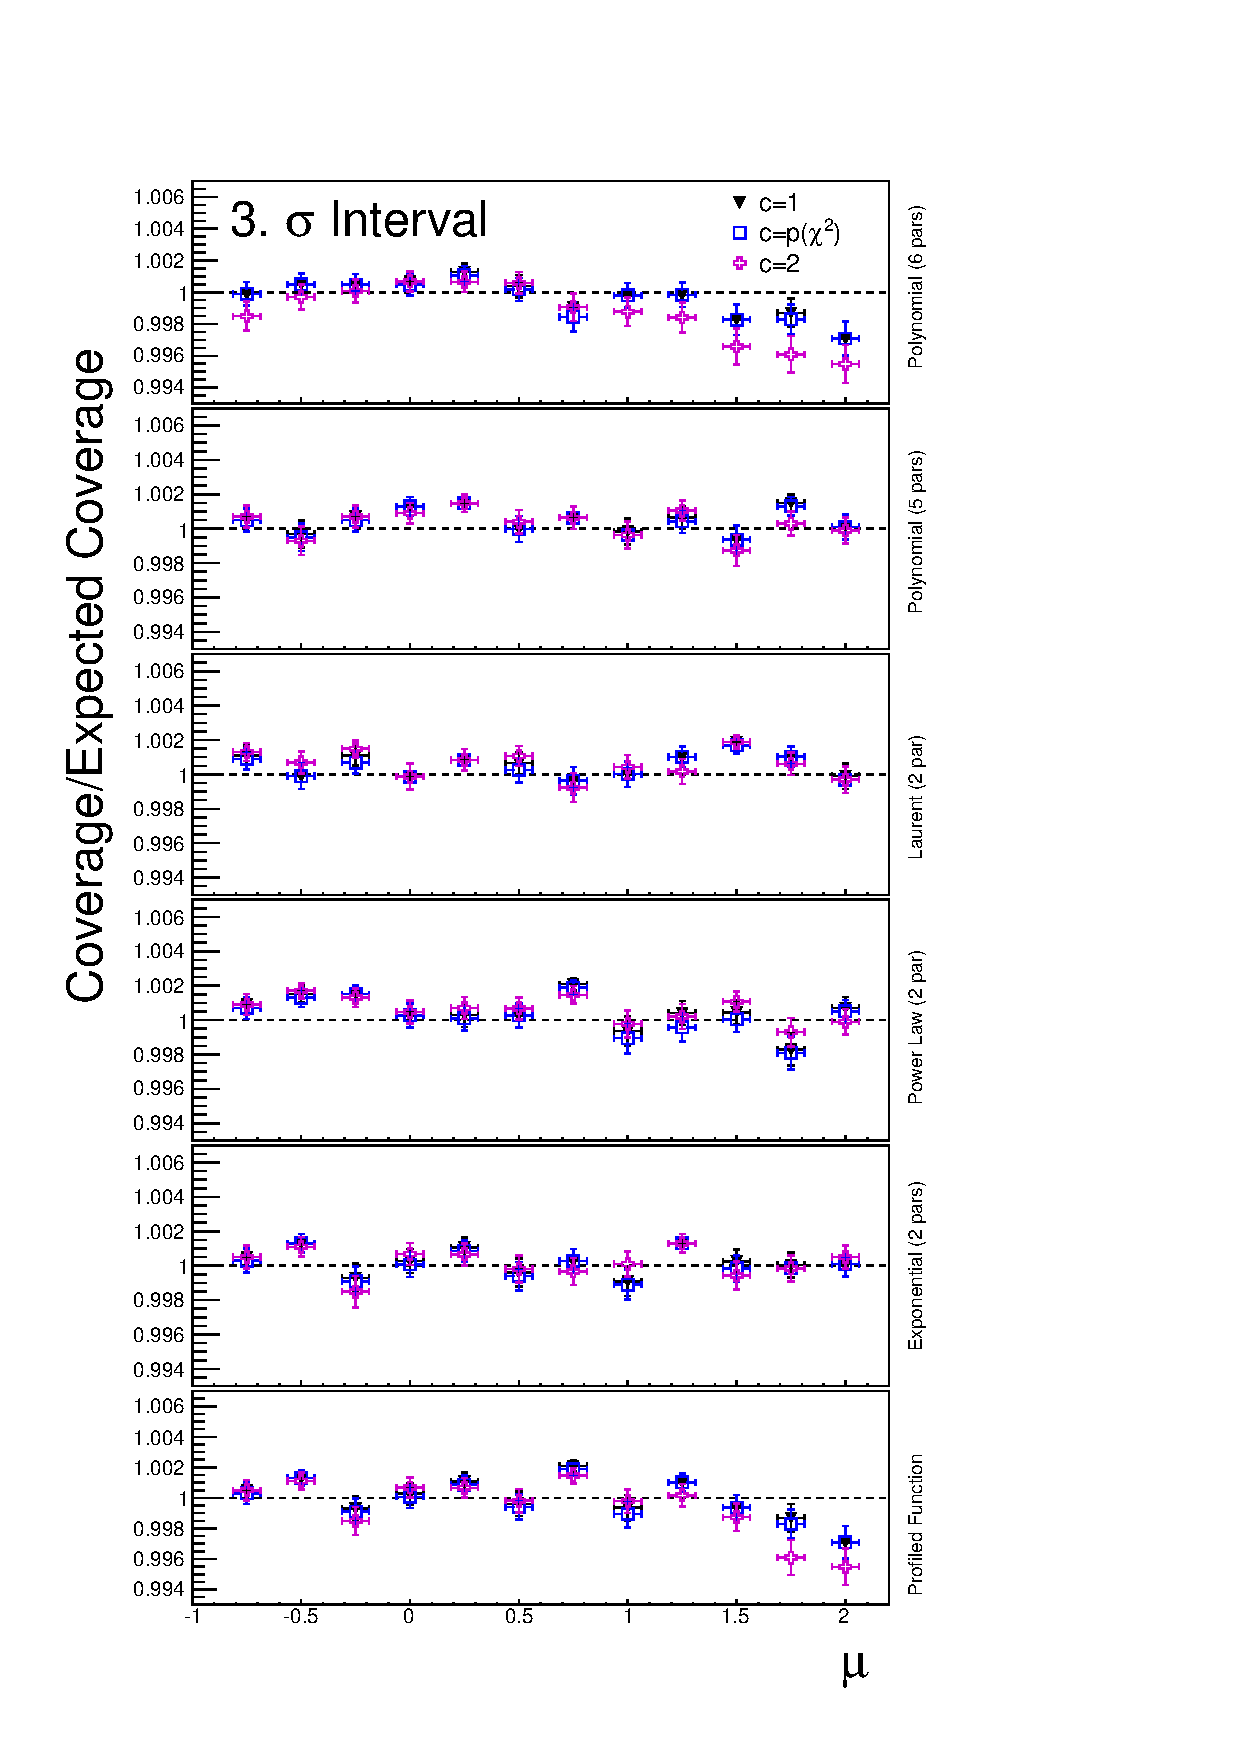
\includegraphics[width=0.45\textwidth]{{correction/AllOrderFunctions_Coverage_3._call}.pdf}
\caption{Fraction of toys in which the fitted value of $\mu$ is within the 0.5, 1, 2 and 
$3\sigma$ intervals relative to the expected fraction for that iterval when correcting 
with the different 2NLL correction schemes. 
The results when generating with different functions and generating using the 
profiled function for each value of $\mu$ are shown in the different panels.  }
\label{fig:correction:allordercoverage}
\end{figure}
%BIAS VS CORRECTION

%ERROR VS CORRECTION.

%DOES BIAS $\rightarrow 0$ for CORRECTION $\rightarrow 0$?
